\documentclass[border=10pt]{standalone}
\usepackage{tikz}\usepackage{amsmath}\usetikzlibrary{arrows.meta}
\begin{document}
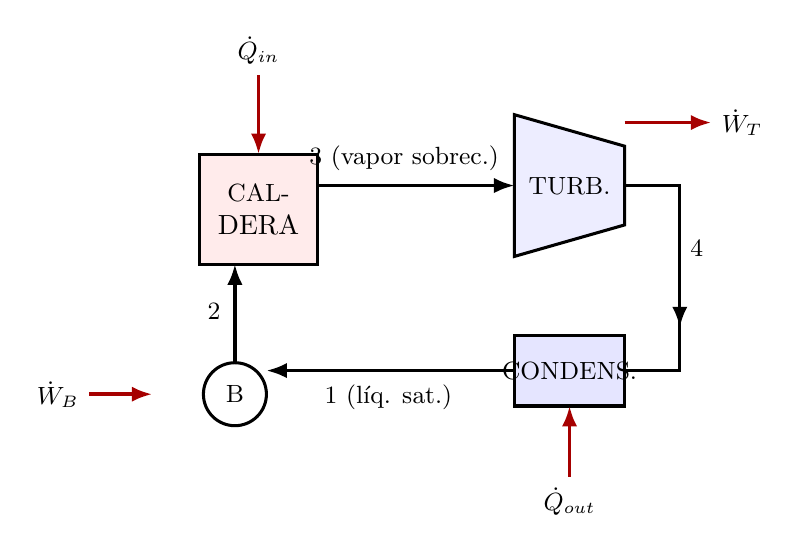
\begin{tikzpicture}[line width=1pt,>={Latex[length=2.6mm]}]
  % --- componentes ---
  \fill[red!8] (0,1.8) rectangle (1.5,3.2); \draw[line width=1.1pt] (0,1.8) rectangle (1.5,3.2);
  \node[align=center] at (0.75,2.5){\small CAL-\\DERA};
  \fill[blue!7] (4.0,1.9)--(5.4,2.3)--(5.4,3.3)--(4.0,3.7)--cycle;
  \draw[line width=1.1pt] (4.0,1.9)--(5.4,2.3)--(5.4,3.3)--(4.0,3.7)--cycle;
  \node at (4.7,2.8){\small TURB.};
  \fill[blue!10] (4.0,0) rectangle (5.4,0.9); \draw[line width=1.1pt] (4.0,0) rectangle (5.4,0.9);
  \node at (4.7,0.45){\small CONDENS.};
  \draw[line width=1.1pt] (0.45,0.15) circle (0.4); \node at (0.45,0.15){\small B};
  % --- tuberias (sentido horario) ---
  \draw[->,line width=1.2pt] (1.5,2.8)--(4.0,2.8); \node[above] at (2.6,2.85){\small 3 (vapor sobrec.)};
  \draw[line width=1.2pt] (5.4,2.8)--(6.1,2.8)--(6.1,0.45)--(5.4,0.45);
  \draw[->,line width=1.2pt] (6.1,1.8)--(6.1,1.0); \node[right] at (6.1,2.0){\small 4};
  \draw[->,line width=1.2pt] (4.0,0.45)--(0.85,0.45); \node[below] at (2.4,0.4){\small 1 (líq. sat.)};
  \draw[->,line width=1.2pt] (0.45,0.55)--(0.45,1.8); \node[left] at (0.4,1.2){\small 2};
  % --- interacciones ---
  \draw[->,red!65!black,line width=1.3pt] (0.75,4.2)--(0.75,3.2); \node[above] at (0.75,4.2){\small $\dot Q_{in}$};
  \draw[->,red!65!black,line width=1.3pt] (4.7,-0.9)--(4.7,0); \node[below] at (4.7,-0.9){\small $\dot Q_{out}$};
  \draw[->,red!65!black,line width=1.3pt] (5.4,3.6)--(6.5,3.6); \node[right] at (6.5,3.6){\small $\dot W_T$};
  \draw[<-,red!65!black,line width=1.3pt] (-0.6,0.15)--(-1.4,0.15); \node[left] at (-1.4,0.15){\small $\dot W_B$};
\end{tikzpicture}
\end{document}
